\documentclass[11pt]{article}

\usepackage[RGB,dvipsnames]{xcolor}
\usepackage[colorlinks=true,pdftex]{hyperref}
\hypersetup{
     citecolor=blue,urlcolor=blue
           }
\usepackage{graphicx}
\usepackage[nottoc,numbib]{tocbibind} 
\usepackage{enumitem}
\usepackage[top=0in, bottom=1in, left=1in, right=1in]{geometry}
\usepackage{caption} 



\usepackage{listings}
\usepackage{color}

\definecolor{dkgreen}{rgb}{0,0.6,0}
\definecolor{gray}{rgb}{0.5,0.5,0.5}
\definecolor{mauve}{rgb}{0.58,0,0.82}

\lstset{frame=tb,
  language=HTML,
  aboveskip=3mm,
  belowskip=3mm,
  showstringspaces=false,
  columns=flexible,
  basicstyle={\small\ttfamily},
  numbers=none,
  numberstyle=\tiny\color{gray},
  keywordstyle=\color{blue},
  commentstyle=\color{dkgreen},
  stringstyle=\color{mauve},
  breaklines=true,
  breakatwhitespace=true
  tabsize=3
}

\definecolor{SnotGreen}{rgb}{0,0.9,0}
\usepackage[authoryear]{natbib}

\begin{document}
\begin{titlepage}

\title{
      Report on the Development of a WebSite for the National Skeptics Association using Ruby-on-Rails (v3.2)\\
        }   
\author{%
Thomas Dowling$^{1}$\\ 
(x12113441)\\\\
    $^{1}$National College of Ireland.\\ \\
	  Web Application Frameworks\\
	  M.Sc in Web Technologies\\\\
	  Lecturer: Jonathan McCarthy
	  }	
	
\maketitle
\vspace*{125px}
\begin{figure}[h!]
\centering
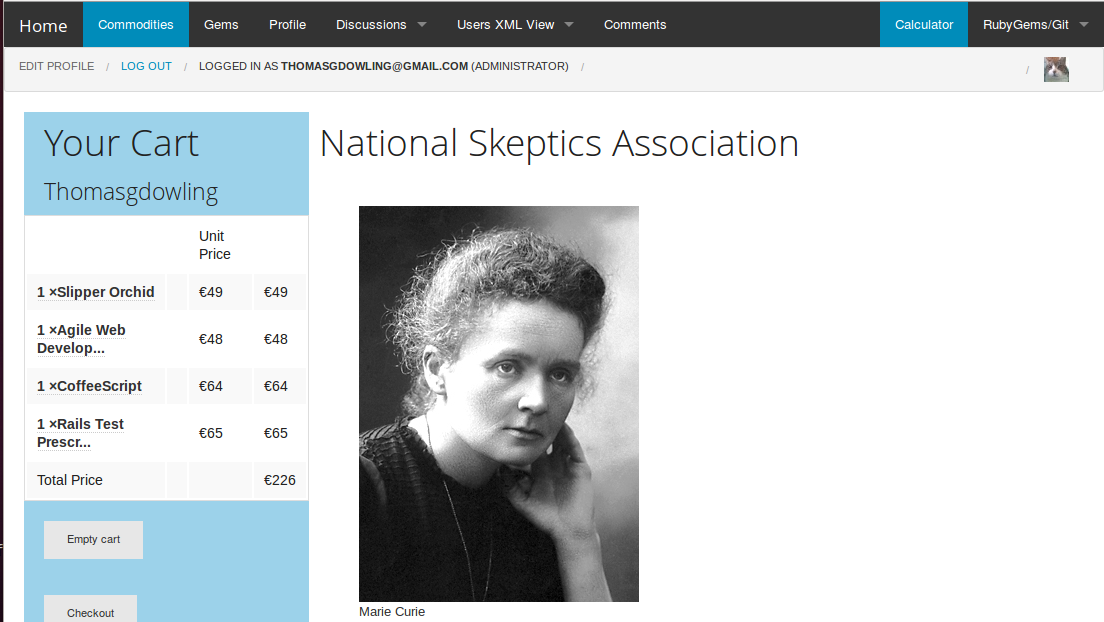
\includegraphics[scale=0.3]{./images/skepticsOne.png}
\end{figure}
\hypersetup{linkcolor=OliveGreen}
\newgeometry{top=0.5in, bottom=1in, left=1in, right=1in}
\clearpage
\tableofcontents

\end{titlepage}
\hypersetup{linkcolor=OliveGreen}
\newgeometry{top=0.5in, bottom=1in, left=1in, right=1in}

\hypertarget{label:sectMEINTRO}{ \section{Introduction}\label{label:meintro}}

The goal of the project was to build a web site for a fictional society, the National Skeptics Association, with the following
requirements. 
\begin{itemize}
\item[] It was desired that the site would have log-in facilities where three types of user were envisaged: An unregistered user,
a registered user and an administrator. An unregistered user should be encouraged to register, but should be able to browser the site with restricted privileges even while not registered. 
\item[]A registered  user should be able to log-in with an email address and password, be able to update
that password, and be able to easily generate a new password from a lost-password request. 
\item[]It was envisaged that the site would have full e-commerce functionality that allows a user to purchase 
products from a Commodities page. The Commodities page should be searchable. 
\item[]In addition, a shopping cart should be visible on every page that allows a user to easily add and delete items,
to at all times see the quantity, price and total cost of all items purchased, and to proceed to checkout. A key requirement
is that the shopping card be user-friendly.  The cart should not be visible unless an item has been added, but a registered user
should be aware when the cart is empty.  
\item[] When a registered user makes a purchase from the Checkout page, she/he should receive an email message detailing the items purchased
\item[] The name of a logged-in user should appear on the nav-bar, together with the status of that user (administrator or non-administrator). 
\item[] A registered user's Gravatar should appear on the nav-bar.
\item[]When a new user registers, her/his details should be appended to an XML file that may be viewed dynamically from
a web page by a user with administration status (and only by such a user).

\item[]In addition, an administrator should be able to view a formatted version of the 'raw' XML file. 
\item[] All registered users should have a Profile page which the user may edit. In addition, a registered user should be able
to upload an image to the Profile page, and edit that image if desired. A registered user should only have access to his/her Profile page. 
\item[] It was also a requirement that a user with administration status could create Discussion pages, upload images to the
Discussion pages, and edit the pages. 
\item[]In addition, registered users may leave comments on the Discussion pages which will  be visible to all users as soon
as posted. A registered user should be able to edit his/her own comments \textbf{but not those of another user}.   
An administrator should be able to view, search, edit and delete all comments. 
\item[] It was desired that the database be protected from invalid and incomplete entries.
\end{itemize}

This report outlines how the above requirements were implemented. 





  








\hypertarget{label:sectmeARCH}{ \section{Architecture}\label{label:mearch}}

The architecture of the site, as viewed from the point of view of a user browsing to the home
page, is shown in \hyperlink{label:figsitemap}{Fig. 1}
It is largely self-explanatory, but a couple of point require comment.
\begin{itemize}
\item[] An unregistered user will have access to all pages except the Profile, Comments, Shopping Cart, Checkout,
Dynamic XML and Static XML pages. In addition, an unregistered user may not leave comments (but may read the comments
of other users), and may not purchase products (but may search the database of Commodities). 
\item[] Upon registration, a user will have access to an automatically generated Profile page (which may be edited), may
purchase commodities, and may leave comments. A registered user without administrator status will not have access to the
Comments page, the Dynamic XML Page, or view the static ('raw') XML file.   
\item[] An administrator has access to all pages. 
\end{itemize}

\begin{figure}[h!]
\centering
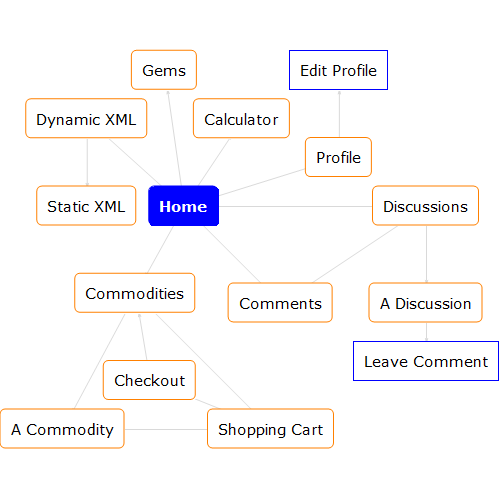
\includegraphics[scale=0.6]{./images/sitemap.png}
\label{label:sitemap}
\hypertarget{label:figsitemap}{\caption{Site Architecture as Viewed From Home Page}}
\end{figure}





\hypertarget{label:sectmeGENIMP}{ \section{General Implementation Methods}\label{label:megenimp}}




\subsection{Programs and Frameworks}



\begin{itemize}[itemsep=1ex,leftmargin=1cm,rightmargin=1cm]
\item[] The website was developed using Ruby(v 1.9.3p0) 
as the primary programming language
and Ruby-on-Rails (v 3.2.14) as framework.

\item[]A 'skeleton front-end' was created
using the 
\href{http://zurb.com/}{Zurb Foundation}
CSS framework.   
\item[]JavaScript was used primarily to
create dynamic content integrated with an  XMLHttp request (to dynamically display
a list of users from an XML file). 
\item[] jQuery was used in Ajax requests (see below, \hyperlink{label:sectajax}{Section~\ref{label:ajax}})
\item[] jQuery-UI was used to add advanced functionality features,
such as making the shopping cart HTML div draggable. 
\item[] The 
\href{https://rubygems.org/gems/mailcatcher/}{Mailcatcher} 
gem was used to 'catch' emails (issued when the user purchased a product, say) 
in development mode.  
\item[] The \href{http://rubygems.org/gems/paperclip}{Paperclip}
gem was used to allow users to upload photographs to a profile page, and to allow
administrators to upload images to the Discussion forums. 
\item[] The application was built on a Dell PC with Ubuntu 12.04 as operating system. 
\end{itemize}



 
\subsection{External Gems}
The gems following gems were used

\begin{itemize}[itemsep=1ex,leftmargin=1cm,rightmargin=1cm]
\item[] \textbf{\href{https://rubygems.org/gems/annotate}{annotate}}
 Annotates Rails models based on the database schema
\item[] \textbf{\href{https://github.com/mislav/will_paginate/wiki}{will-paginate}} Advanced pagination functionality for Rails.
\item[] \textbf{\href{https://rubygems.org/gems/faker}{faker}} Allows the generation of 'fake' data
\item[]\href{http://zurb.com/}{foundation-rails} Installs the Zurb-Foundation CSS framework
\item[] \textbf{\href{https://github.com/joliss/jquery-ui-rails}{jquery-ui-rails}} Makes advanced jQuery features available 
\item[] \textbf{\href{https://github.com/plataformatec/devise}{devise}} Advanced user authentication functionality
\item[] \textbf{\href{http://rubygems.org/gems/nokogiri}{nokogiri}} Generate and sort XML files
\item[] \textbf{\href{https://github.com/mdeering/gravatar_image_tag}{gravatar-image-tag}} Displays a user's gravatar 
\item[] \textbf{\href{http://rubygems.org/gems/paperclip}{paperclip}}  Allows user to easily upload images. \href{http://www.imagemagick.org/script/index.php}{ImageMagick} must be installed
for full functionality 
\item[] \textbf{\href{https://github.com/rspec/rspec-rails}{rspec-rails}} Advanced test-driven development 
\item[] \textbf{\href{http://rubygems.org/gems/mail}{mail}}  Great mailer functionality becomes available 
\item[] \textbf{\href{https://rubygems.org/gems/mailcatcher/}{mailcatcher}}  Allows emails to be 'caught' in 
development mode.
May be accessed via port 1080 (localhost:1080). 
\item[] \textbf{\href{http://rubygems.org/gems/figaro}{figaro}} Rails configuration using ENV and a YAML file (used in conjunction with the \href{http://rubygems.org/gems/mail}{mail} gem)

\end{itemize} 




 
\subsection{Gems developed in this Work}
Three gems were created in this project, and published on RubyGems. 
All may be included in the Gem file of a Rails application and installed 
using the \verb| bundle install| command.

\begin{itemize}[itemsep=1ex,leftmargin=1cm,rightmargin=1cm]

\item[] \textbf{\href{https://rubygems.org/gems/jscalc}{JavaScript Calculator(jscalc)}}

This gem was created using a Rails engine 
(\verb|Rails::Engine|) method and
allows a JavaScript calculator (written by \href{http://mathematica.stackexchange.com/users/106/tomd}{Tom Dowling}) to be incorporated into a Rails application. 
(The engine method allows the incorporation of `mini-apps' into gems).

\href{https://rubygems.org/gems/jscalc}{jscalc}
 has so far been downloaded more than 1300 times from \href{https://rubygems.org/}{RubyGems}. 
In the present work, a clash with \href{http://zurb.com/}{Zurb-Foundation} CSS (which added unwanted classes to the buttons)
was solved by incorporating the calculator into a web page with a separate controller and a separate
layout file (\verb|jscalc.html.erb|). One attraction of 
\href{https://rubygems.org/gems/jscalc}{jscalc}
 is that it accepts JavaScript functions, 
such as \verb|Math.random()|, as input.

A version of \href{https://rubygems.org/gems/jscalc}{jscalc} in a basic Rails application is also available at
\url{http://tgd-jscalc.herokuapp.com/} 

\item[] \textbf{\href{https://rubygems.org/gems/binToDec}{Binary to Decimal Converter (binToDec)}}

This gem provides the functionality to convert a binary number to a decimal.
If the argument provided is not binary, an exception is thrown. It has been unit-tested. 

When the gem is installed, the following functionality becomes available.

\begin{verbatim}
  Converter.binToDec(arg)
\end{verbatim}

The program uses the following code to test if the input is binary.

\begin{verbatim}
  arg1.to_s.split(//)
      .map { |i| i.to_i }
        .find_all { |value| value > 0 }
          .inject(:*)
\end{verbatim}

If the test passes the input is converted to binary with the following function.
\begin{verbatim}
    arg1.to_s
      .split(//)
        .map { |i| i.to_i }
          .inject(0) { |accumulator, value| (accumulator + value) * 2 }

    return result/2
\end{verbatim}
\href{https://rubygems.org/gems/binToDec}{binToDec} has been downloaded more that 750 times from \href{https://rubygems.org/}{RubyGems}.    
\item[] \textbf{\href{https://rubygems.org/gems/priceMarkup}{Cost Price to Formatted Selling Price (priceMarkUp)}}

This gem allows the selling price to be calculated from the cost price based on a markup. 

The default markup is 0.25. 

In addition, the number of decimal places in the output may be specified. 
When the gem is installed, the following functionality becomes available.
\begin{verbatim}
   Dowstore.priceMarkup(price, markup, decimal_places)
\end{verbatim}

Examples of usage are as follows
\begin{verbatim}
   Dowstore.priceMarkup(100) => "125"
\end{verbatim}

\begin{verbatim}
   Dowstore.priceMarkup(100, 2) => "300"
\end{verbatim}
\begin{verbatim}
   Dowstore.priceMarkup(100, 2, 3) => "300.000"
\end{verbatim}
Extensive use of \href{https://rubygems.org/gems/priceMarkup}{priceMarkUp} 
has been made during the course of this work. It has been unit-tested.
\end{itemize} 

\hypertarget{label:sectajax}{ \subsection{Ajax}\label{label:ajax}}
Two methods were used to incorporate Ajax requests.

\begin{itemize}[itemsep=1ex,leftmargin=1cm,rightmargin=1cm]
\item[] The fist method used the jQuery  \verb|$.ajax()| method to set up the XMLHttp request and
is based on the method learned in lectures. It was used primarily to `Ajax-enable' nav-bar links
(so that when a user clicks on such a link the whole page is not renewed via a new HTTP request,
but the relevant content is `injected' into the current page using an Ajax request). 
\item[] The second method uses the `Rails way' as outlined, for example, in \textit{Agile Web Development with Rails} \cite[pp 136 - 139]{agile2012}.

Briefly the method used was as follows. 
Say a nav-bar contains a link to a page rendered from the index method of a controller,
and it is desired to Ajax-enable that link. In the example below this is the index action of the
\verb|comments_controller|.  
\begin{enumerate}
\item The \verb|remote: true| parameter is passed to the link as shown:
\begin{verbatim}
<%= link_to "Comments", comments_path, remote: true %>
\end{verbatim}
\item The line `\verb|format.js|' is added to the \verb|index| method of the \verb|comments_controller| so that it
reads as follows.
\begin{verbatim}
  respond_to do |format|
      format.html # index.html.erb
      format.js
      format.json { render json: @comments }
\end{verbatim}
\item In views, a  partial is made (in the same directory) of \verb|index.html.erb| (called \verb|_index.html.erb|)
\item Also in the same directory, a file called \verb|index.js.erb| 
is created and jQuery is used to render the partial. Typically, the \verb|.js.erb| 
file contained code something like the following (where \verb|#yieldId| is the id of a div (in \verb|application.html.erb|) 
containing the \verb| <%= yield %> | command:
\begin{verbatim}
$(`#yieldId').html(`<%=j render partial: `comments/index' %>');
\end{verbatim}  

\end{enumerate} 
The \textit{j} is important, as it invokes the \textit{j}() helper method which converts a Ruby string to a form
compatible with JavaScript \citep[p 138] {agile2012}.
 
This method was used quite a lot to add Ajax functionality to the application.  
As well as nav-bar links, it was used for example to Ajax-enable 
the addition of items to the shopping cart (so that when an item is placed in the cart by a user a separate
HTTP request is not sent).
\end{itemize}




\hypertarget{label:sectappendsort}{ \subsection{Append to and Sort an XML file when a New User Registers}\label{label:appendsort}}

Two functions, \verb|builder()| and \verb|myAdd()| (within a module called \verb|TGD|), were
written that
generate relevant XML tags (\verb|builder|), 
add content to those tags, 
append the populated tags to a well-formed XML file,
and sort it alphabetically such that the updated file is also well-formed (\verb|myAdd|).

When called from the create action of a relevant controller,
these functions may be used to update and sort an XML file
every time a new user registers.

An abridged version of the code is shown in \hyperlink{label:figxmlfns}{Fig. 2}  
The unabridged version may be found in \verb|lib/xmlfunctions.rb | in the \textit{skeptics}
Rails application. 
 
In the present work, \verb|TGD.myAdd()| was called
from the \verb|create| action of the 

\noindent
\verb|registrations_controller|, and
\verb|public/xmlNewUsers.xml| is updated when a new user registers.

Functionality provided by the  \href{http://rubygems.org/gems/nokogiri}{nokogiri} gem was incorporated into
both functions to help generate and insert the XML tags, 
and to sort the XML file. 

The XML file to be updated must exist, 
and must contains a root directory called \verb|root|. 
The reason for this is that \verb|myAdd()| removes the closing tag
from the open XML file 

\noindent
(\verb|f.seek(-8, IO::SEEK_END)|) 
before appending the new contents 
\textbf{together with a new closing root tag}. 
The file need minimally
contain \verb|<root>|
     \verb|</root>|, but of course it may also be populated with XML data
and contain DTD meta-data in the Head section.


\begin{figure}[ht!] 
\begin{verbatim}
     
module TGD
  def self.builder (my_username, my_id, ...)
    Nokogiri::XML::Builder.new do |xml|
      xml.myUsers do |xml|
        xml.email my_username;
        xml.userID my_id;
        ...
      end
    end
  end

  def self.myadd(email,my2id, ... filename)
#xml file must have a root-directory called root
    f = File.open(filename, "r+")
    f.seek(-8, IO::SEEK_END)
    f << builder(email,my2id ...)
    .to_xml(:save_with => Nokogiri::XML::Node::SaveOptions::NO_DECLARATION)
    f<< "</root>"
    f.close
    f = File.open(filename)
    doc = Nokogiri::XML(f) do |config|
      config.options = Nokogiri::XML::ParseOptions::NOBLANKS
    end
    node1 = doc.at_xpath(`//root')
    sorted = node1.children.sort_by{ |n| n.text }
    sorted.each{ |n| node1 << n }
    file = File.open(filename,`w')
    file.puts doc.to_xml
    file.close
  end
end
\end{verbatim}
\label{label:xmlfns}
\hypertarget{label:figxmlfns}{\caption{Append to and Sort an XML file (xmlfunctions.rb, abridged)}}

\end{figure}






\hypertarget{label:secthttpz}{ \subsection{Use XMLHttp Request to View an XML File Dynamically}\label{label:httpz}}
In order to to display an XML file on a web-page dynamically,
a set of functions (/app/assets/javascripts/tgdxmlHTTP.js) were 
written which, at their core, use an XMLHttp request to retrieve 
data from an XML file. In addition, JavaScript was used to create
a series of buttons that allow a user to dynamically browse the
contents of the file. A user may advance one entry, go back one entry,
go forward or back five entries, to to the beginning of the file,
or go to the end of the file (\hyperlink{label:figdypict}{Fig. 3}).
In the present work, this functionality was used to allow browsing of
the newUsers.xml file discussed in the previous section (\hyperlink{label:sectappendsort}{Section~\ref{label:appendsort}}).
When
a new user registers, the relevant data are added to /public/xmlNewUsers.xml, 
and the (alphabetically sorted) entry may immediately be viewed on a
web page. 
This functionality has been restricted to a user with administration status.
 
\begin{figure}
\centering
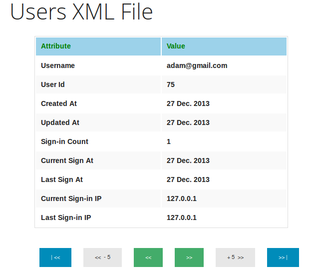
\includegraphics[scale=1]{./images/dxml.png}
\hypertarget{label:figdypict}{\caption{Dynamic XML File Functionality in a Web Page}}
\label{label:dypict}
\end{figure}




\subsection{Validation}
To protect the database from invalid date entry, the
Orders,
Commodities and
Discussion 
models were validated using Rails validation. 
For example:
\begin{verbatim}



   validates   :name,
               :category,            
               :description,            
               :price,
               :presence => true

   validates :price,
               :numericality => {:greater_than_or_equal_to => 1 }
               
  \end{verbatim}          


\subsection{Mailers}
The functionality provided by the \href{http://rubygems.org/gems/mail}{mail} gem was
used to set up a mailer (mailers/order\_notifier.rb) 
that sends a formatted email
to a registered user 
when commodities are purchased via the Checkout page.
The formatted email contains the price and quantity of each product. 

In addition, the \href{https://github.com/plataformatec/devise}{Devise} mailer has been set up so that
a user receives an email when the `Forgot Password?' link is clicked on
the log-in menu. 
Clicking on the link within the email brings the user to the
 \href{https://github.com/plataformatec/devise}{Devise} Change Password 
page, and allows the password to be changed.

For development purposes, the emails are `caught' by
\href{https://rubygems.org/gems/mailcatcher/}{Mailcatcher}
but it is  easy to change the setting so that emails are sent to (say) gmail 
(three relatively simple changes in config/environment.rb). 

\href{https://rubygems.org/gems/mailcatcher/}{Mailcatcher} may be accessed on port 1080 (localhost:1080)

\subsection{Unit Testing and Test-Driven Development}
Unit tests were written to test the functionality of both
the 
\href{https://rubygems.org/gems/jscalc}{binToDec} 
and 
\href{https://rubygems.org/gems/priceMarkup}{priceMarkup} 
gems.

 
For example (test\_binToDec in the \href{https://rubygems.org/gems/jscalc}{jscalc} gems directory)

\begin{verbatim}
# Test if an valid binary number given an incorrect value
  def test_binary_false
    assert_not_equal 9,
    Converter.binToDec(1000)
  end
\end{verbatim}
\begin{verbatim}
# Test if an invalid binary number raises an exception
def test_non_binary_true
  
  assert_raise RuntimeError do
  Converter.binToDec(2222)
    end
  end
\end{verbatim}
In addition, 
\href{http://rspec.info/}{RSpec} was installed and some
preliminary TDD tests were written. 
A mistake make here is that
\href{http://rspec.info/}{RSpec}
 should have been installed at the beginning of the project, rather
than towards the end. 

An example of an \href{http://rspec.info/}{RSpec} test for the commoditites\_controller is the following (spec/controllers/commodities\_controller\_spec.rb): 
\begin{verbatim}
describe CommoditiesController do

  describe "GET `index'" do
    it "returns http success" do
      get 'index'
      response.should be_success
    end

    it `should have a non-blank body' do
      get `index'
      response.body.should_not =~ /<body>\s*<\/body>/
    end
  end
  ...
end
\end{verbatim}
\subsection{Paperclip and Image Upload}
\href{http://rubygems.org/gems/paperclip}{Paperclip}, 
in conjunction with 
\href{http://www.imagemagick.org/script/index.php}{ImageMagick}, 
was used to
provide two pieces of image-upload functionality.
\begin{itemize}
\item[] Users may upload a image to their Profile page, or
edit that image, by browsing from a Paperclip-provided link  
on the Devise Sign-Up and Edit-User pages.
The uploaded image appears correctly formatted on the Profile page.
\item[] An administrator may upload or edit images on the Discussion
pages. The uploaded image appears on the relevant Discussions Page and and as
a thumbnail on the Index page of the Discussions Model.
\end{itemize}
It was observed that \href{http://rubygems.org/gems/paperclip}{Paperclip}  is a lot easier to use (almost flawless)
on an Ubuntu OS, 
compared with Windows (where, in the experience of this
user, it is very difficult to get to work properly). 
\subsection{Search}
\begin{itemize}
\item[] Search functionality was incorporated into the 
Commodities/index page,
Comments/index page and
Discussions/index page.


\item[] On the Commodites/index page
a user may choose,
by radio-button selection,
whether to search by name,
by category or by description,
or by all of the above criteria (default). 

\end{itemize}
\subsection{Will-paginate}

\href{https://github.com/mislav/will_paginate/wiki}{Will-pagination} was used for pagination of tables 
and for pagination of search results on the Comments/index, Discussions/index and Commodites/index pages.

\href{http://mislav.uniqpath.com/will_paginate/}{Digg pagination} (CSS) was used for formatting. 
In the opinion of this user, \href{https://github.com/mislav/will_paginate/wiki}{Will-pagination} is one of
the very best gems. 

\subsection{Devise}
The \href{https://github.com/plataformatec/devise}{Devise} gem was used for user authentication. 
An \href{https://github.com/plataformatec/devise/wiki/How-To:-Add-an-Admin-role}{administrator role}
was added to the basic installation.
\begin{itemize}
\item[] A user may log-in using an email address. 
The user is asked to confirm address.
\item[] An administrator may log in (and gain
additional privileges).
\item [] A user may change her/his password 
via a link sent to the user's email account
\item[] A user may update her/his profile
\item[] A registrations\_controller was created in 
order to allow data to be appended to an XML file when
a new user registered (called from the def/create action of
the registrations\_controller).
\item[] A users\_controller was added allow users to create a
profile (def/show) and to add authentication functionality
\end{itemize}
\subsection{Gravatars}
The \href{https://github.com/mdeering/gravatar_image_tag}{Gravatar Image Tag} was installed a Ruby gem
and was used to display
the Gravatar of a registered user on the `breadcrumbs' nav-bar.
If a registered user does not have a Gravatar, a default image is displayed. 
\subsection{Before Filtering}
The \verb|before_filter| method was used to restrict access to controller actions.

For example, to allow only a registered user to access his/her Profile page but not the
Profile page of any other registered user, and in addition to allow an administrator to
access (via the nav-bar) the Profile page of any user, the following code was added 
to the users\_controller.

\begin{verbatim}
    before_filter :validate_user
    
	 def validate_user
    		redirect_to root_path unless current_user 
                          and current_user.id.to_s == params[:id] 
                          or current_user.admin
     end
\end{verbatim}
\hypertarget{label:sectmeSPIMP}{ \section{Specific Implementation Components}\label{label:mespimp}}
\subsection{Shopping Cart/Commodities Page}
A lot of effort was put into integrating the Shopping Cart and Commodities Page
and these will be taken together.
\begin{itemize}
\item[] Only a registered user may purchase items. 
An unregistered user may, however, view and search the list of commodities
\item[] The shopping cart is only visible when a registered user adds an item to it.  When the
Cart is empty, a div with the message `Your Cart is empty' is displayed. (This is done using
\verb|hidden_div_if| and \verb|hidden_div_unless| methods in application\_helper.rb).
\item[] A user may add items by clicking on the `Add to Cart` button 
\textbf{or by clicking on the image of the product}.
\item[] The Shopping Cart (rendered as a partial) is visible on every page as long as it is not empty. This 
includes the Checkout page.
\item[] When a user adds an item to the Cart, the price of the item, the quantity and total
price are immediately displayed in the Cart, and these are dynamically updated every time a user adds a product.
\item[] Adding a product to the cart, either by clicking on the button or the image, are `Ajax-enabled'. That is, only
the Cart portion of the page is updated and \textbf{a separate HTTP request is NOT sent for every item purchased}.
\item[] When an item is added to the Cart, a green background fades in and then fades out in that line-item, indicating
to the user that an item has been successfully added. 
\item[] A user may delete individual items from the Cart (by hovering over the line item), or delete the whole Cart.
\item[] The Cart may be made smaller by clicking on the `Smaller' button.  When this is done, only the total price is
displayed, and the user is given the options of going to Checkout or making the Cart larger again.
  
Making the Cart smaller is done with an Ajax request. When the `Smaller' button is clicked a new partial is rendered 
showing a smaller cart. (Unfortunately, making the Cart larger has not been Ajax-enabled). 
\item[] The Cart is draggable (done with jQuery-UI). 
\item[] The `humanized' name of the registered user appears at the top of the Cart
\item[] Only an administrator may Edit and Destroy items on the Commodities Page. 
\end{itemize}
\subsection{Check-out}
When the user click the `Check Out' button on the Cart, he/she is taken to
the Checkout page and invited to fill in details such as first name, last name
email address, credit card type. The user must also confirm the email address and
Rails validation is used to ensure that the two emails match (\verb|validates| \verb|:email_confirmation| in
the Orders Model).
\begin{itemize}
\item[] When the User successfully fills in the form and clicks `Purchase', he or she receives
a formatted email message (send to the address supplied) showing details of the  items purchased.
\item[] The Cart is emptied
\item[] The user is redirected to the Commodities Page and receives a message `Thank you for your order'.
\end{itemize}
\subsection{Dynamic Users XML File}
The dynamic display of the Users XML file has been discussed in
 \hyperlink{label:secthttpz}{Section~\ref{label:httpz}}. Here it need only be added that this functionality is restricted
to a user with administrator status. 
\subsection{Static Users XML File}
By clicking on a link in on the Dynamic Users XML view page, an administrator may
view (in a separate page) a formatted version of the `raw' XML file(\verb|xmlNewUsers.xml|).  Formatting was
done using an XML-transform (see /public/\verb|xmlNewUsers.xsl|). 
\subsection{Profile Pages}
When a user registers, a Profile page is automatically created.
\begin{itemize}
\item[] A user may upload an image to his/her Profile Page
\item[] A user may edit his/her Profile page (including the image)
\item[] The Profile page displays the image uploaded by the user together
with user details. For example:
\begin{verbatim}

E-mail 	thomasgdowling@gmail.com
Human Name 	Thomasgdowling
User Id 	51
User Created At 	25 Dec. 2013
User Updated At 	01 Jan. 2014
Sign-in Count 	28
Current Sign in On 	01 Jan. 2014
Last Sign-in On 	31 Dec. 2013
Current IP 	127.0.0.1
Last Sign-in IP 	127.0.0.1

\end{verbatim}
\end{itemize}
\subsection{Discussion Pages and User Comments}

Discussion Pages are created by an administrator, but a registered user
may leave comments
\begin{itemize}
\item[] Only a registered user may leave a comment
\item[] When a user leaves a comment, it is immediately visible on the relevant
\textbf{Discussions page} (not the Comments page) and appears at the top of the paginated list.
\ The length of time since the comment was posted is recorded (time\_ago\_in\_words(comment.created\_at), as is the (humanized)
username. 
\item[] A user may, at any time, destroy or edit his or her comments, \textbf{but not the comments of another user}.
\item[] An administrator may edit and delete all comments (and may administer comments on a separate Comments page).
\item[] A paginated list of all Discussions are shown on a separate Index page. 

\end{itemize}
An example of a user comment is shown in 
\hyperlink{label:figcommeg}{Fig. 4}

\begin{figure}
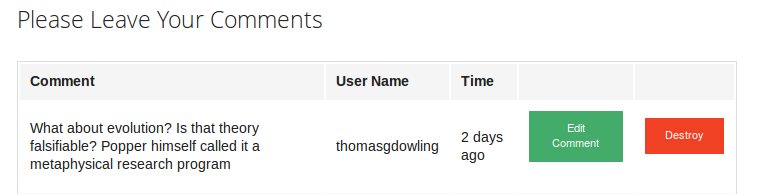
\includegraphics[scale=0.5]{./images/comment.png}
\label{label:commeg}
\hypertarget{label:figcommeg}{\caption{An example of a User Comment}}
\end{figure}


\subsection{Comments Page}

A separate Comments page is provided to allow a user with administrator status
to view all comments, to search the database of Comments, and to Edit or Delete any comment.
\subsection{Authentication Logic}
In order to show certain functionality to a user depending on the registration status of that
user, extensive use was made of the following methods (provided by \href{https://github.com/plataformatec/devise}{Devise})

  \begin{verbatim}
  <% if current_user and current_user.admin %>
  <% if  current_user.present?%>
  <% if current_user.admin? %>
  \end{verbatim}
  

  For example, certain nav-bar items become visible when the user logs in and logs out. In addition,
  the visibility of 'Edit' and 'Destroy' buttons were selectively manipulated using the above methods.
  \section{GitHub and RubyGems}
  \begin{itemize}
  \item[] The code for the skeptics web application is available from \href{https://github.com/tomGdow}{GitHub} at \url{https://github.com/tomGdow/skeptics} 
  
  \item[] The jscalc gem is available at \url{https://rubygems.org/gems/jscalc}
  \item[] The binToDec gem is available at \url{https://rubygems.org/gems/binToDec} 
  \item[] The priceMarkup gem is available at \url{https://rubygems.org/gems/priceMarkup}
  
  \end{itemize}
 \section{Browser} 
 The application is best viewed in a Firefox browser.   
 \section{Discussion} 
 A dynamic, functional web-site for the fictional National Skeptics Association was successfully created using Ruby-on-Rails which incorporated most of the desired functionality. 
 The following observations and criticisms may be made
 \begin{itemize}
 \item[] Rails is a lot easier to use on an Ubuntu operating system, compared to Windows.  This is particularly evident
 with the \href{http://rubygems.org/gems/paperclip}{Paperclip}  gem, which works almost flawlessly with Ubuntu. 
 \item[] RSpec should have been installed earlier in order to avail of the advanced TDD functionality it offers.
 \item [] An Index page showing a list of all users where an administrator can edit and delete user details was not implemented. 
 \item[] The \href{https://github.com/plataformatec/devise}{Devise} gem is an excellent method for providing authorization functionality. 
 \item[] There was a `clash' between the \href{https://rubygems.org/gems/jscalc}{jscalc} gem developed during the course of this work and \href{http://zurb.com/}{Zurb Foundation} CSS, mainly because Zurb was adding extra classes
 to the buttons, and was adding undesired formatting to the input box. There seems no easy way around this as it 
does not seem to be possible to protect a button from this type of class `injection'. However, this problem  needs to be sorted, and
the solution posted to RubyGems. 
\item[] Will-pagination is an excellent gem
\item[] A method needs to be implemented that allows searching of the XML file from a web page. 
\item[] In addition, a method needs to 
be implemented that allows `purging' of all data except the root directory from the XML file.  In this way, an administrator could
record in an XML file the details of users who register in a given time period (and browse the XML data dynamically). 
 \end{itemize}
\hypertarget{label:sectmeDEC}{ \section{Declaration}\label{label:medec}}

I hereby certify that this material, which I now submit for assessment of the program of study leading to the award of Master of Science in Web Technologies is entirely my own work and has not been taken from the work of others save and to the extent that such work has been cited and acknowledged within the text of my work.

\vspace*{15px}
\noindent
Thomas Dowling (x12113441)

\bibliographystyle{agsm-tgd}
\hypersetup{linkcolor=blue}
\bibliography{skeptics.bib}
\hphantom{M}
\hphantom{M}

\end{document}
